\documentclass[14pt]{extarticle}
\usepackage{graphicx}
\usepackage{amsmath}
\usepackage{xcolor}





\begin{document}

\title{Sicurezza}
\author{Alessandro Savioli}
\date{Marzo 2025}

\maketitle

\tableofcontents

\newpage

\section{Introduzione}

Secondo il \textbf{NIST} (National Institute of Standards and Technology) il
termine \textit{sicurezza informatica} può essere definito come:

\begin{center}
    Misure e controlli che assicurino \textbf{confidenzialità, integrità e
    disponibilità} di asset del sistema informatico che includono hardware,
    software, firmware e informazioni processate, memorizzate e comunicate.
\end{center}

\section{CIA e Livelli di impatto}

\subsection{CIA}

Nel campo della sicurezza informatica possiamo trovare tre \\ obiettivi o
requisiti principali:

\begin{itemize}
    \item \textbf{Confidentiality}, ovvero preservare l'accesso autorizzato e
    prevenire la divulgazione di informazioni, come dati sensibili o
    proprietari;
    \item \textbf{Integrity}, ovvero la prevenzione contro la modifica o \\ la
    distruzione impropria di informazioni, assicurando anche che un informazione
    non possa essere ripudiata oltre che quest'ultima sia autentica;
    \item \textbf{Availability}, ovvero assicurare l'accesso ad una determinata
    informazione.  
\end{itemize}

A questi tre obiettivi principali se ne possono accostare ulteriori due, così da
formare un quadro completo di tutto ciò che serve ad un sistema per essere
sicuro:

\begin{itemize}
    \item \textbf{Authenticity}, ovvero la proprietà di un utente di essere
    verificato e affidabile. Questo significa verificare che gli utenti siano
    chi dicono di essere e che gli input del sistema derivino sempre da una
    fonte affidabile;
    \item \textbf{Accountability}, ovvero la capacità di tracciare le attività
    di una qualsiasi entità all'interno del sistema, così da poter ricondurre un
    attacco ad un responsabile e tenere traccia di cosa sia successo per andare
    poi a migliorare la sicurezza del sistema. 
\end{itemize}

\begin{center}
    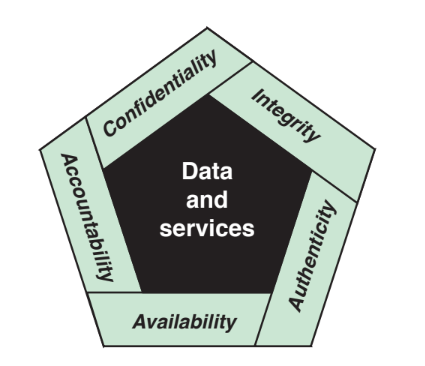
\includegraphics{images/CIA.png}
\end{center}

\newpage
\subsection{Livelli d'impatto}

Analizziamo ora i diversi livelli d'impatto che un attacco può procurare ad una
organizzazione:

\begin{enumerate}
    
    \item \textbf{Impatto basso}, causa una degradazione lieve alle funzioni \\
    dell'organizzazione, che risulta ancora in grado di svolgere le sue funzioni
    principali ma con efficacia ridotta. Può causare danni \textbf{minori} ad
    assets, finanze o danni agli individui;
    \item \textbf{Impatto moderato}, causa una degradazione significativa alle
    funzioni dell'organizzazione, che risulta ancora in grado di svolgere le
    proprie funzioni ma con efficacia nettamente ridotta. Può causare danni
    \textbf{significativi} ad assets e finanze o agli individui, senza includere
    perdite di vite;
    \item \textbf{Impatto elevato}, causa una degradazione severa alle funzioni
    dell'organizzazione, che non risulta più in grado di svolgere una o più
    delle sue funzioni primarie. Può causare danni \textbf{severi o
    catastrofici} ad assets e finanze o agli individui, includendo anche perdite
    di vite. 

\end{enumerate}

\subsection{Un modello per la sicurezza informatica}

\begin{center}
    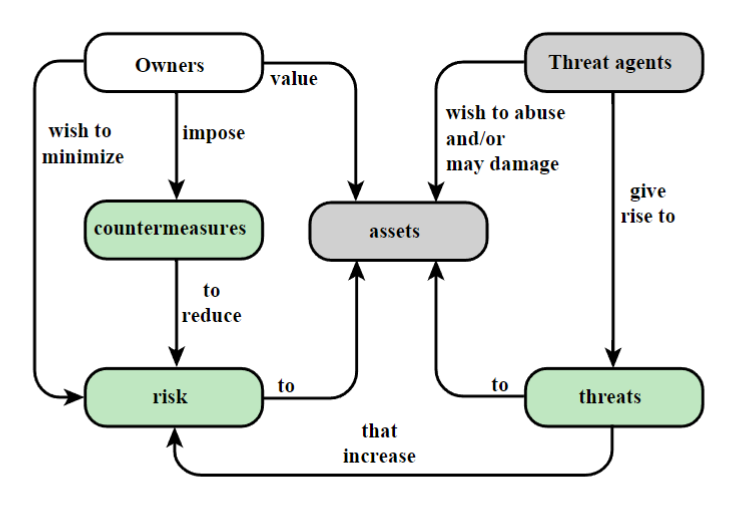
\includegraphics[scale=0.78]{images/modello.png}
\end{center}

\noindent Diamo ora alcune nozioni su termini di base nella sicurezza
informatica:

\begin{itemize}
    \item \textbf{Systes Resource (Asset)}, che può essere hardware, software,
    dati o reti;
    \item \textbf{Vulnerability (di un asset)}, ovvero una debolezza nel sistema
    informatico, nelle procedure di sicurezza, controlli interni o
    nell'implementazione che potrebbe essere superata da un attacco. Possiamo
    distinguere 3 principali debolezze, in quanto un sistema può essere:
    \textbf{Corrupted, Leaky, Unavaiable};
    \item \textbf{Threat (minaccia)}, ovvero ogni circostanza o evento con il
    potenziale di avere un impatto negativo verso l'organizzazione o anche
    specifiche funzioni;
    \item \textbf{Adversary (threat agent)}, ovvero un individuo, un gruppo o
    una organizzazione che conduce o ha l'intento di condurre un attacco;
    \item \textbf{Attack}, qualsiasi tipo di attività malevola che prova a
    ottenere, distruggere, vietare o modificare le risorse di un sistema
    informatico o il sistema informatico stesso;
    \item \textbf{Countermeasure}, uno strumento o delle tecniche che hanno come
    obiettivo di proteggere o prevenire attacchi informatici;
    \item \textbf{Risk}, una misura che indica il rischio che una risorsa venga
    attaccata, che risulta essere il prodotto tra l'impatto negativo che si
    avrebbe se questa risorsa fosse attaccata e la probabilità che questo
    succeda;
    \item \textbf{Security Policy}, un insieme di criteri standard per la
    sicurezza di sistemi informatici o risorse.     
\end{itemize}

\subsection{Attacchi e Conseguenze}

Possiamo suddividere le conseguenze di un attacco in 4 tipi:
\begin{enumerate}
    \item Rilascio non autorizzato;
    \item Inganno;
    \item Interruzione;
    \item Usurpazione.
\end{enumerate}

Cerchiamo di vederli nel dettagli e capire quali sono gli attacchi che possono
portare a queste conseguenze:

\subsubsection{Rilascio non autorizzato}

Il rilascio non autorizzato si verifica quando un'entità non autorizzata ottiene
l'accesso ad informazioni. Gli attacchi che portano a questa conseguenza possono
essere di tipo:
\begin{itemize}
    \item \textbf{Exposure}, in cui un utente autorizzato invia direttamente
    delle informazioni ad un utente non autorizzato;
    \item \textbf{Interception}, in cui un utente non autorizzato accede a delle
    informazioni che stanno passando in rete tra due utenti autorizzati;
    \item \textbf{Inference}, in cui un utente non autorizzato ottiene
    indirettamente l'accesso a dei dati grazie a delle caratteristiche o scarti
    della comunicazione;
    \item \textbf{Intrusion}, in un utente non autorizzato ottiene l'accesso a
    dei dati dopo aver superato le protezioni di sicurezza.   
\end{itemize}

\subsubsection{Inganno}

L'inganno si verifica quando un'entità autorizzata riceve una falsa informazione
credendo che sia vera. Gli attacchi che portano a questa conseguenza sono di
tipo:
\begin{itemize}
    \item \textbf{Masquerade}, in cui un'entità non autorizzata ottiene
    l'accesso al sistema e si finge un utente autorizzato;
    \item \textbf{Falsification}, in cui false informazioni ingannano un'entità
    autorizzata;
    \item \textbf{Repudiation}, in cui un'entità ne inganna un'altra negando la
    responsabilità di un'azione ingiustamente.  
\end{itemize}

\subsubsection{Interruzione}

Un'interruzione si verifica quando un attacco blocca il corretto funzionamento
dei servizi di un sistema. Gli attacchi che portano a questa conseguenza sono di
tipo:
\begin{itemize}
    \item \textbf{Incapacitation}, interrompe una o più funzioni di sistema
    disabilitando un componente di sistema;
    \item \textbf{Corruption}, altera le operazioni di sistema modificando delle
    funzioni o i dati;
    \item \textbf{Obstruction}, interrompe i servizi di sistema ostacolando le
    operazioni.    
\end{itemize}

\subsubsection{Usurpazione}

Un'usurpazione si verifica quando un'entità non autorizzata prende il controllo
del sistema o di alcune funzioni di esso. Gli attacchi che portano a questa
conseguenza sono di tipo:
\begin{itemize}
    \item \textbf{Misappropiation}, in cui un'entità assume il controllo fisico
    o logico non autorizzato di una risorsa di sistema;
    \item \textbf{Misuse}, in cui si spinge un componente di sistema a svolgere
    azioni che abbassano il livello di sicurezza del sistema. 
\end{itemize}

\subsection{Attacchi passivi e attivi}



\end{document}